\section{Previous research}
\label{sec:kernel_previous_research}

Before presenting our model for estimating social mixing patterns using ARD, it is important to review previous work in estimating social mixing. These methodologies were created as byproducts of trying to more accurately estimate personal network size via the scale-up method \citep{Killworth+others:1998}.

To gain an intuition for the scale-up method, consider a population of size $N$. We can store the information about the social network connecting the population in an adjacency matrix $\triangle = [\delta_{ij}]_{NxN}$ such that $\delta_{ij} = 1$ if person $i$ knows person $j$. Throughout this paper we will assume the \citet{McCarty+others:2001} definition of know: "that you know them and they know you by sight or by name, that you could contact them, that they live within the United States, and that there has been some contact (either in person, by telephone or mail) in the past 2 years." The personal network size or degree of person $i$ is then $d_i =  \sum_j \delta_{ij}$.

Since it is unrealistic to ask survey respondents whether they know every single individual in the population, the \citet{Killworth+others:1998} scale-up method uses responses to ARD to estimate personal network size. For example, if you report knowing 3 women who gave birth, this represents about one-millionth of all women who gave birth within the last year. Assuming that your personal network's demographics are similar to that of the whole country, we can then use this information to estimate that you know about one-millionth of all Americans,
\begin{equation}
\frac{3}{3.6 \text{ million}} \cdot (300 \text{ million}) \approx 250 \text{ people}. 
\end{equation} 

As such, in Section \ref{subsec:overdispersion} we present an earlier model by \citet{Zheng+others:2006} that formalizes an overdispersion framework of the scale-up method, accounting for the variation in propensity to know individuals from certain subpopulations. This overdispersion framework, while providing a probabilistic interpretation of the scale-up method, suffers from transmission errors and barrier effects. In Section \ref{subsec:mixing_matrix} we present a more recent model by \citet{McCormick+others:2010} that addresses these issues, and as a byproduct allows estimation of the mixing patterns between age and gender groups.

% Zheng 2006 Overdispersion Model
\subsection{The \citet{Zheng+others:2006} model with overdispersion}
\label{subsec:overdispersion}

The multilevel overdispersed Poisson model of \citet{Zheng+others:2006} was the first to treat random mixing as something important to estimate for its own sake. 

Let $y_{ik}$ denote the number of people that person $i$ knows in subpopulation $\scriptG_k$, $N_k$ denote he size of subpopulation $\scriptG_k$, and $N$ denote the size of the population. \citet{Zheng+others:2006} noted that under simple random mixing the responses to the ARD questions, $y_{ik}$'s, would follow a Poisson distribution with rate parameter determined by the degree of person $i$, $d_i$, and the network prevalence of group $\scriptG_k$, $b_k$:
\begin{align}
y_{ik} &\sim \text{Poisson}(\lambda_{ik}) && \\\nonumber
\lambda_{ik} &= f(d_i, b_k).
\end{align}
Here $b_k$ is the proportion of ties that involve individuals in subpopulation $k$ in the entire social network. If we can assume that individuals in the group being asked about (e.g. people named Michael), on average, as popular as the rest of the population, then $b_k \approx N_k/N$.

Like \citet{Killworth+others:1998} before, \citet{Zheng+others:2006} used the telephone survey conducted by \citet{McCarty+others:2001} to test the above hypothesis. The responses to many of the questions in the survey data did not follow a Poisson distribution, however. In fact, most of the responses show overdispersion (i.e. excess variance given the mean). For example, consider the responses to the question: "How many males do you know incarcerated in state or federal prison?" The mean of the responses to this question was 1.0, but the variance was 8.0, indicating that some people are much more likely to know someone in prison than others. To model this increased variance \citet{Zheng+others:2006} allowed individuals to vary in their propensity to form ties to different groups. If these propensities follow a gamma distribution with a mean value of 1 and a shape parameter of $1/(\omega_k-1)$ then the $y_{ik}$ can be modeled with a negative binomial distribution,
\begin{align}
y_{ik} &\sim \text{Neg-Binom}(\text{mean} = \mu_{ik}, \text{overdispersion} = \omega_k). && \label{eq:overdispersion}
\end{align}
Thus, the $\omega_k$ estimate the variation in individual propensities to form ties to people in different groups and represent one way of quantifying non-random mixing. 

Then, letting $\{i \to j\}$ denote the event that ego $i$ knows alter $j$ and letting $\{j \in \scriptG_k\}$ denote the event that alter $j$ is a member of subpopulation $\scriptG_k$, the expected number of people known in subpopulation $\scriptG_k$ by ego $i$ with degree $d_i$ can be derived as
\begin{align}
\mu_{ik} 
&= \ex \biggl[ \sum_{j=1}^{d_i} \ind\{ j \in \scriptG_k \} \biggr] && \\\nonumber
&= \sum_{j=1}^{d_i} \ex \biggl[ \ind\{ j \in \scriptG_k \} \biggl| i \to j \biggr] && \\\nonumber
&= \sum_{j=1}^{d_i} \prob( j \in \scriptG_k | i \to j) && \\\nonumber
&= d_i \prob( j \in \scriptG_k | i \to j) && \\\nonumber
&= d_i \biggl( \frac{N_k}{N} \biggr).
\end{align}
Consequently, in addition to estimating $\omega_k$, this model also produces personal network size estimates, $d_i$, but this methodology has a couple drawbacks. First, this framework does not provide estimation of the dependence of social mixing on inherent agent characteristics, such as age or gender. Secondly, the degree estimates from this model are susceptible to biases due to transmission errors and barrier effects. 

Transmission errors occur when a respondent knows someone in a subpopulation, but is not aware that the alter is actually in that subpopulation. For example, a respondent might know a man who has prostate cancer, but might not know that he has prostate cancer. Certain subpopulations may have higher rates of transmission errors due to reasons such as social stigma (e.g. women who have had an abortion) or political reasons (e.g. men who are in the NRA). In general, these errors are difficult to quantify because the amount of information respondents have about their connections is unknown \citep{Killworth+others:2006}. 

Barrier effects occur whenever some individuals systematically know more (or fewer) members of a specific subpopulation than would be expected under random mixing (i.e. non-random mixing). For example, since people tend to know others of similar age and gender \citep{McPherson+others:2001}, a 25-year old woman probably knows more women who have recently had an abortion than would be predicted just based on her personal network size and the number of women who have had an abortion. Similarly, an 80-year old man probably knows fewer than would be expected under random mixing. 

% McCormick 2010 Non-Random Mixing Model
\subsection{The \citet{McCormick+others:2010} non-random mixing model}
\label{subsec:mixing_matrix}

\citet{McCormick+others:2010} resolved the issues found in the \citet{Zheng+others:2006} overdispersion model by making a couple important improvements. First, they restricted their analysis of ARD to questions in which $\scriptG_k$ are only first names. This removed transmission errors, a common problem in previous ARD studies, because individual $i$ must know individual $j$'s name if $j$ is indeed "known" by $i$ under the \citet{McCarty+others:2001} definition. Most crucially, however, \citet{McCormick+others:2010} allowed the expected number known $\mu_{ik}$ to depend not on the overall prevalence of $\scriptG_k$ in the network, but specifically on the prevalence of $\scriptG_k$ within specific age and gender demographics. Combining these subprevalences with the known age and gender of the respondents, \citet{McCormick+others:2010} were then able to effectively remove barrier effects as well.

Specifically, by assuming that egos of certain ages and genders mix differently with alters of other ages and genders, the \citet{McCormick+others:2010} framework models non-random mixing by age and gender. The mixing patterns are modeled by first letting each individual $i$'s age $\scriptA_i$ belong to a discrete age category
\begin{align}
\scriptA_i \in  \{0-20, 21-40, 41-60, 61+\}. \label{eq:mix_age_cat}
\end{align}
Additionally, an individual $i$'s gender $g_i$ is allowed to take on one of two numeric values
\begin{align}
g_i &= 
\begin{cases}
1 & \text{if individual } i \text{ is female}  \\
2 & \text{if individual } i \text{ is male} .
\end{cases} \label{eq:mix_gender_cat}
\end{align}
With these quantities defined, the probability of alter $j$ being in age category $\scriptA_j$ and gender $g_j$, given that ego $i$ in age category $\scriptA_i$ and gender $g_i$ knows alter $j$ ($\{i \to j\}$), becomes
\begin{align}
p(\scriptA_j, g_j | \scriptA_i, g_i, i \to j)
&= M_{[(\scriptA_i,g_i),(\scriptA_j,g_j)]}, && \label{eq:nonrandom_mixing_matrix}
\end{align}
where $M_{[(\scriptA_i,g_i),(\scriptA_j,g_j)]}$ is the mixing rate between egos with gender $g_i$ in age category $\scriptA_i$ and alters with gender $g_j$ in age category $\scriptA_j$. In other words, $100 \times M_{[(\scriptA_i,g_i),(\scriptA_j,g_j)]}$\% of the personal network of an ego with gender $g_i$ and age category $\scriptA_i$ is expected be composed of alters with gender $g_j$ and age category $\scriptA_j$.

Treating $M_{[(\scriptA_i,g_i),(\scriptA_j,g_j)]}$ as elements of a matrix $M$, the rows of $M$ are then constrained to sum to $1$ with
\begin{align}
\sum_{\scriptA_j, g_j} M_{[(\scriptA_i,g_i),(\scriptA_j,g_j)]} &= 1. 
\end{align}

The expected number of people known in $\scriptG_k$ by ego $i$ then becomes
\begin{align}
\mu_{ik} 
&= \sum_{j=1}^{d_i} p( j \in \scriptG_k | \scriptA_i, g_i, i \to j ) && \label{eq:nonrandom_mixing_matrix_derivation} \\\nonumber
&= d_i \prob( j \in \scriptG_k | \scriptA_i, g_i, i \to j) && \\\nonumber
&= d_i \sum_{\scriptA_j,g_j} \prob( j \in \scriptG_k, \scriptA_j, g_j | \scriptA_i, g_i, i \to j) && \\\nonumber
&= d_i \sum_{\scriptA_j,g_j} \prob(\scriptA_j, g_j | \scriptA_i, g_i, i \to j) \prob( j \in \scriptG_k | \scriptA_j, g_j, \scriptA_i, g_i, i \to j) && \\\nonumber
&= d_i \sum_{\scriptA_j,g_j} M_{[(\scriptA_i,g_i),(\scriptA_j,g_j)]}  \prob( j \in \scriptG_k | \scriptA_j, g_j, \scriptA_i, g_i, i \to j) && \\\nonumber
&= d_i \sum_{\scriptA_j,g_j} M_{[(\scriptA_i,g_i),(\scriptA_j,g_j)]} \prob( j \in \scriptG_k | \scriptA_j, g_j)  && \\\nonumber
&= d_i \sum_{\scriptA_j,g_j} M_{[(\scriptA_i,g_i),(\scriptA_j,g_j)]} \biggl( \frac{N_{k, \scriptA_j, g_j}}{N_{\scriptA_j, g_j}} \biggr),
\end{align}
where $N_{k, \scriptA_j, g_j}$ denotes the number of people in subpopulation $\scriptG_k$ and age category $\scriptA_j$ with gender $g_j$, and $N_{\scriptA_j, g_j}$ denotes the number of people in age category $\scriptA_j$ with gender $g_j$.

Since survey respondents are typically required to be 18 years or older, this model generally assumes the existence of 3 ego age categories
\begin{align} 
\scriptA_i \in \{18-24, 25-64, 65+\}, 
\end{align}
4 alter age categories as defined in Equation \ref{eq:mix_age_cat}, and 2 alter and ego genders as defined in Equation \ref{eq:mix_gender_cat}. This results in $M$ being a matrix with $3 \times 2 = 6$ rows and $4 \times 2 = 8$ columns. Accounting for the summation constraints on the rows of $M$, this implies that the non-random mixing model requires estimating $6 \times (7-1) = 42$ independent parameters.

After defining this new framework, \citet{McCormick+others:2010} then applied it to survey responses from \citet{McCarty+others:2001}, estimating not only the individual degrees of the respondents $d_i$ but also the latent non-random mixing matrix $M$. Figure \ref{fig:nonrandom_mixing_matrix} displays the fitted mixing matrix separated by ego age category and gender. The 6 plots correspond to the 6 rows of $M$, while the 8 bars within each plot correspond to the 8 columns of $M$. Most notable is that the alter age distributions for each of the six egos peak at the egos' age categories (i.e. the social networks of young egos are dominated proportionally by young alters, while the social networks of old egos are dominated proportionally by old alters), a phenomenon known as homophily in sociology. The model's ability to estimate homophily without requiring priors on the elements of the mixing matrix is a testament to the power of the latent non-random mixing matrix. 

\begin{figure}
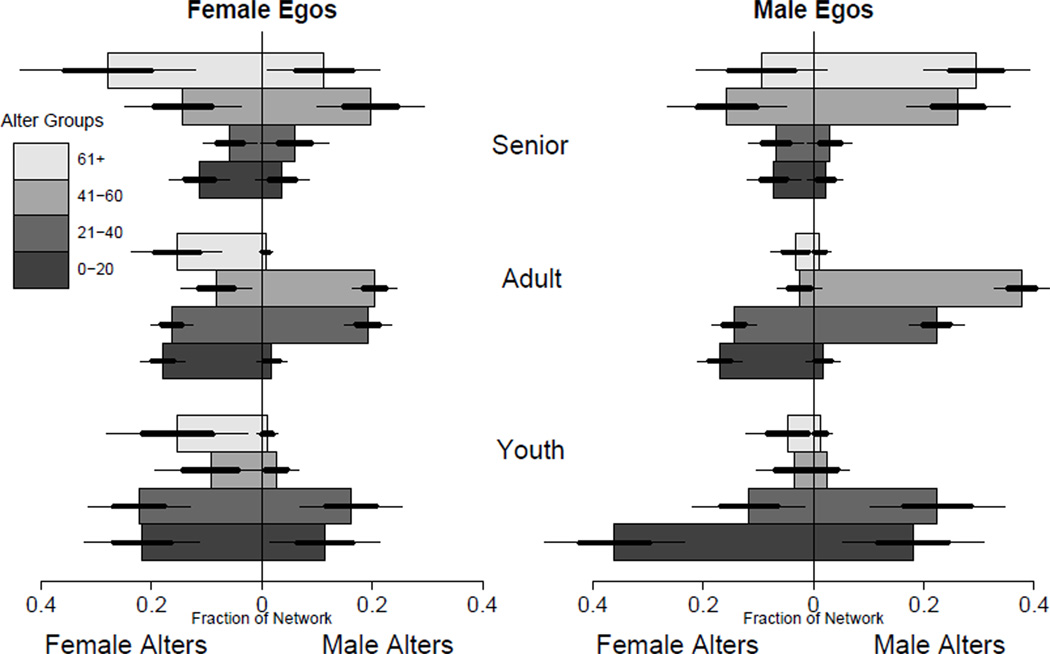
\includegraphics[width=\textwidth]{figures/mccr_latent_mix.jpg}
\caption{The latent non-random mixing matrix estimated from survey respondents who were asked "How many X's do you know?", where X were 12 different names. Each horizontal bar represents the magnitude of an element of the mixing matrix $M_{6 \times 8}$.}
\label{fig:nonrandom_mixing_matrix}
\end{figure}

% Non-Random Mixing Model Simulations Bias Variance
However, this model is not without its faults. In particular, Figure \ref{fig:nonrandom_mixing_matrix} also implies that the all six ego categories know more 0-20 year old females than they do 0-20 year old males, in some cases by several orders of magnitude (e.g., the difference is dramatic for adult egos). This extreme behavior is unexpected, especially given that the national prevalence of males and females is nearly identical amongst 0-20 year olds. While it seems plausible that such a result could be due to the variability of the survey respondents (i.e. perhaps this particular survey's respondents included many individuals who know a lot of young females), our simulated data experiments point to a different explanation. 

\begin{figure}
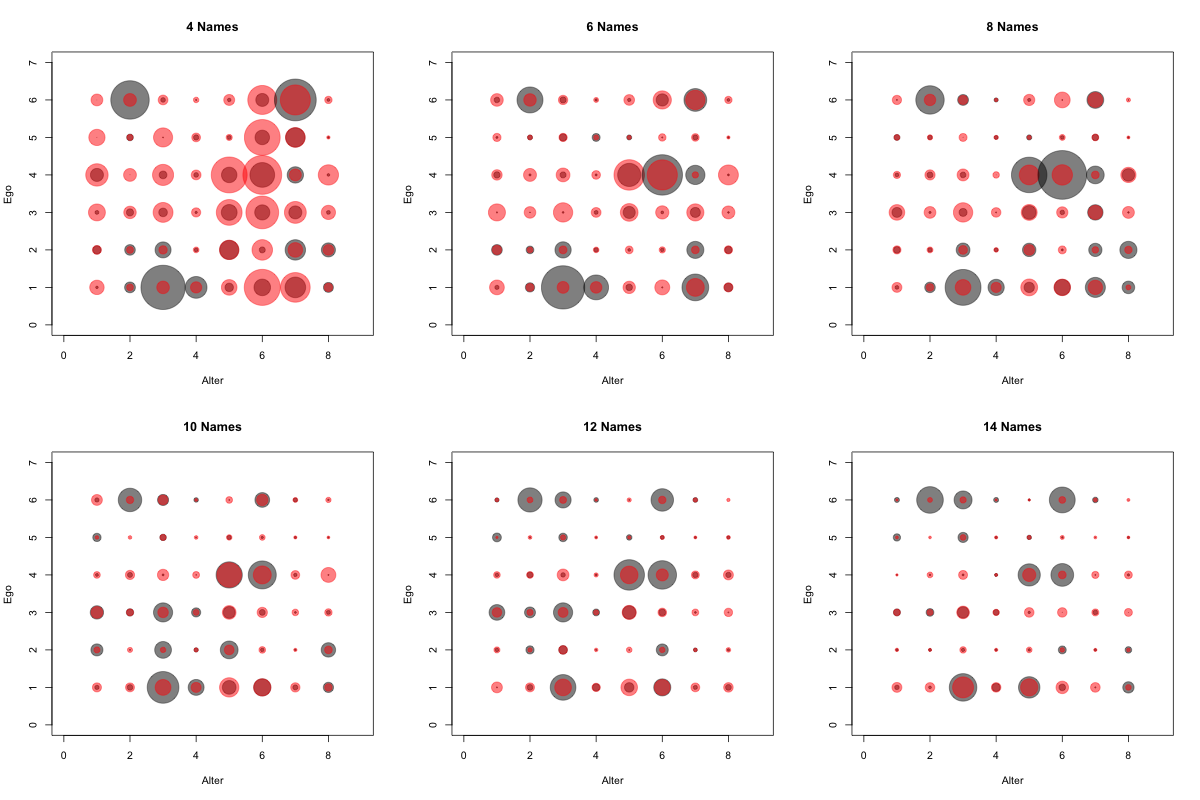
\includegraphics[width=\textwidth]{figures/kernel/matrix/bias_var_1.png}
\caption{The bias and standard error of the posterior mean of each element of the mixing matrix, estimated using simulated responses to 14 names and fitting to 4, 6, 8, 10, 12, and 14 names. The size of the black circles corresponds to bias, and the size of red circles correspond to standard error.}
\label{fig:mixing_matrix_bias_var_1}
\end{figure}

\begin{figure}
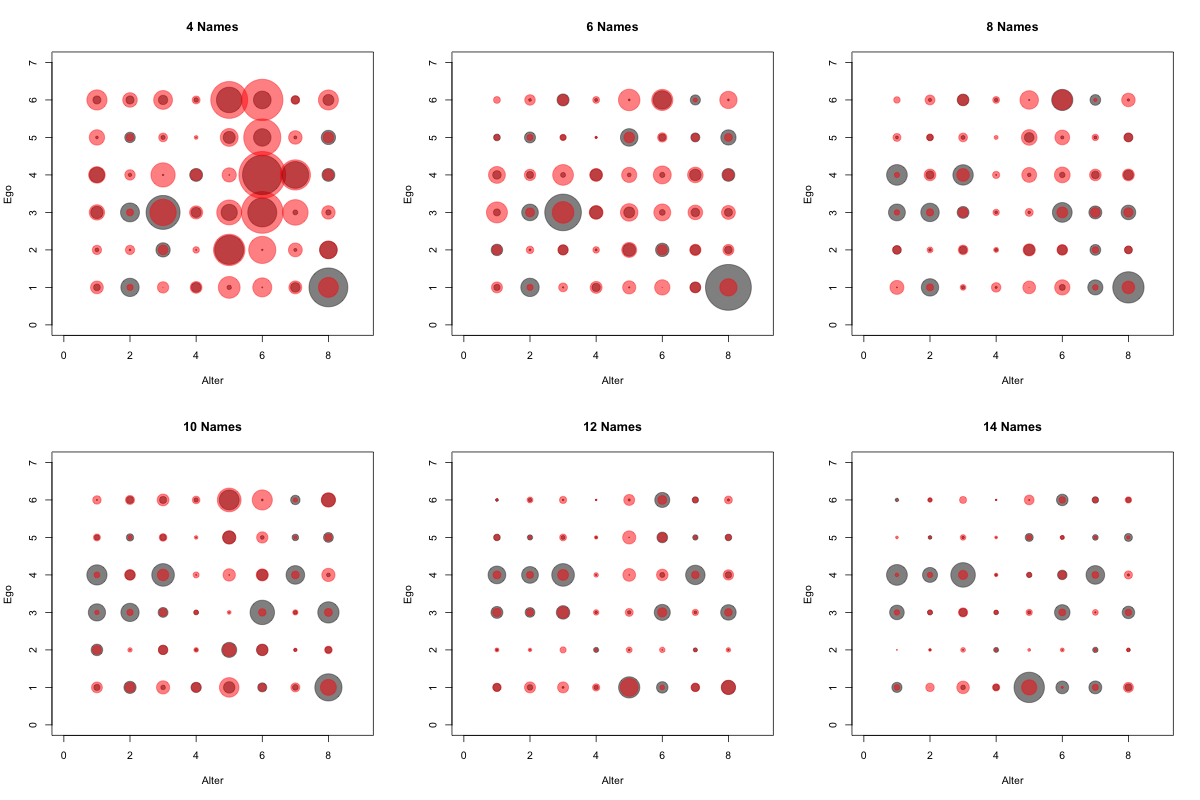
\includegraphics[width=\textwidth]{figures/kernel/matrix/bias_var_3.png}
\caption{The bias and standard error of the posterior mean each element of the mixing matrix, estimated using simulated responses to 14 names and fitting to 4, 6, 8, 10, 12, and 14 names. The size of the black circles corresponds to bias, and the size of red circles correspond to standard error.}
\label{fig:mixing_matrix_bias_var_2}
\end{figure}

Figure \ref{fig:mixing_matrix_bias_var_1} shows the results of constructing a balanced mixing matrix, simulating responses to questions about 14 names, and then trying to recover the mixing matrix by fitting the \citet{McCormick+others:2010} model to a subset of the responses (starting with just 4 names and going up to 14 names). The estimated mixing matrices show extreme biases for certain alter groups, even when using all 14 names. Further still, repeated response simulations from the same fixed mixing matrix produced different posterior estimates of the mixing matrix. Figure \ref{fig:mixing_matrix_bias_var_2} displays the bias and variance of the mixing matrix elements from another set of responses simulated from the same balanced mixing matrix in Figure \ref{fig:mixing_matrix_bias_var_1}. The bias and variance patterns appear sporadic between the two sets of simulations. We believe this is due to the non-identifiability of the mixing proportions, which stems from the lack of structure imposed on $M$'s elements. 
